\section{Introduction}

%从自动驾驶到医疗保健和金融，人工智能正在彻底改变各行各业。然而，要充分发挥人工智能的潜力，就必须将其有效地部署到各种环境中。由于复杂的环境配置、依赖冲突和跨平台适应问题，部署仍然是一个主要瓶颈，阻碍了可扩展性和应用。
%行业中的自动部署主要遵循 DevOps 模式，即使用静态配置文件（如 YAML）定义执行环境、依赖关系和协调规则。在这种方法中，开发人员手动配置环境，指定软件包、版本限制和计算资源分配。然后采用 CI/CD 管道来自动构建、测试和部署。为了提高自动化程度，AutoDevOps 等工具利用预定义模板来简化配置流程。

%然而，这些方法存在不少局限性。首先，缺乏自适应能力，无法基于运行时环境调整部署策略，导致部署仍需人工干预，例如手动调整依赖关系或修复兼容性问题。其次，缺乏经验积累机制，当前的部署方法无法有效记录和复用历史问题的解决方案，导致相同的错误在不同项目或不同阶段重复发生。最后，难以支持复杂任务的模块化复用，传统自动化工具主要针对单一模型的部署，而实际AI应用往往涉及多个模型和系统协同工作，现有方法难以通过标准化接口组合不同组件，限制了AI系统的可扩展性和复用性。这些局限性使得AI部署仍然高度依赖工程经验，阻碍了AI技术的规模化应用。


\begin{figure}[thb]
	\centering
	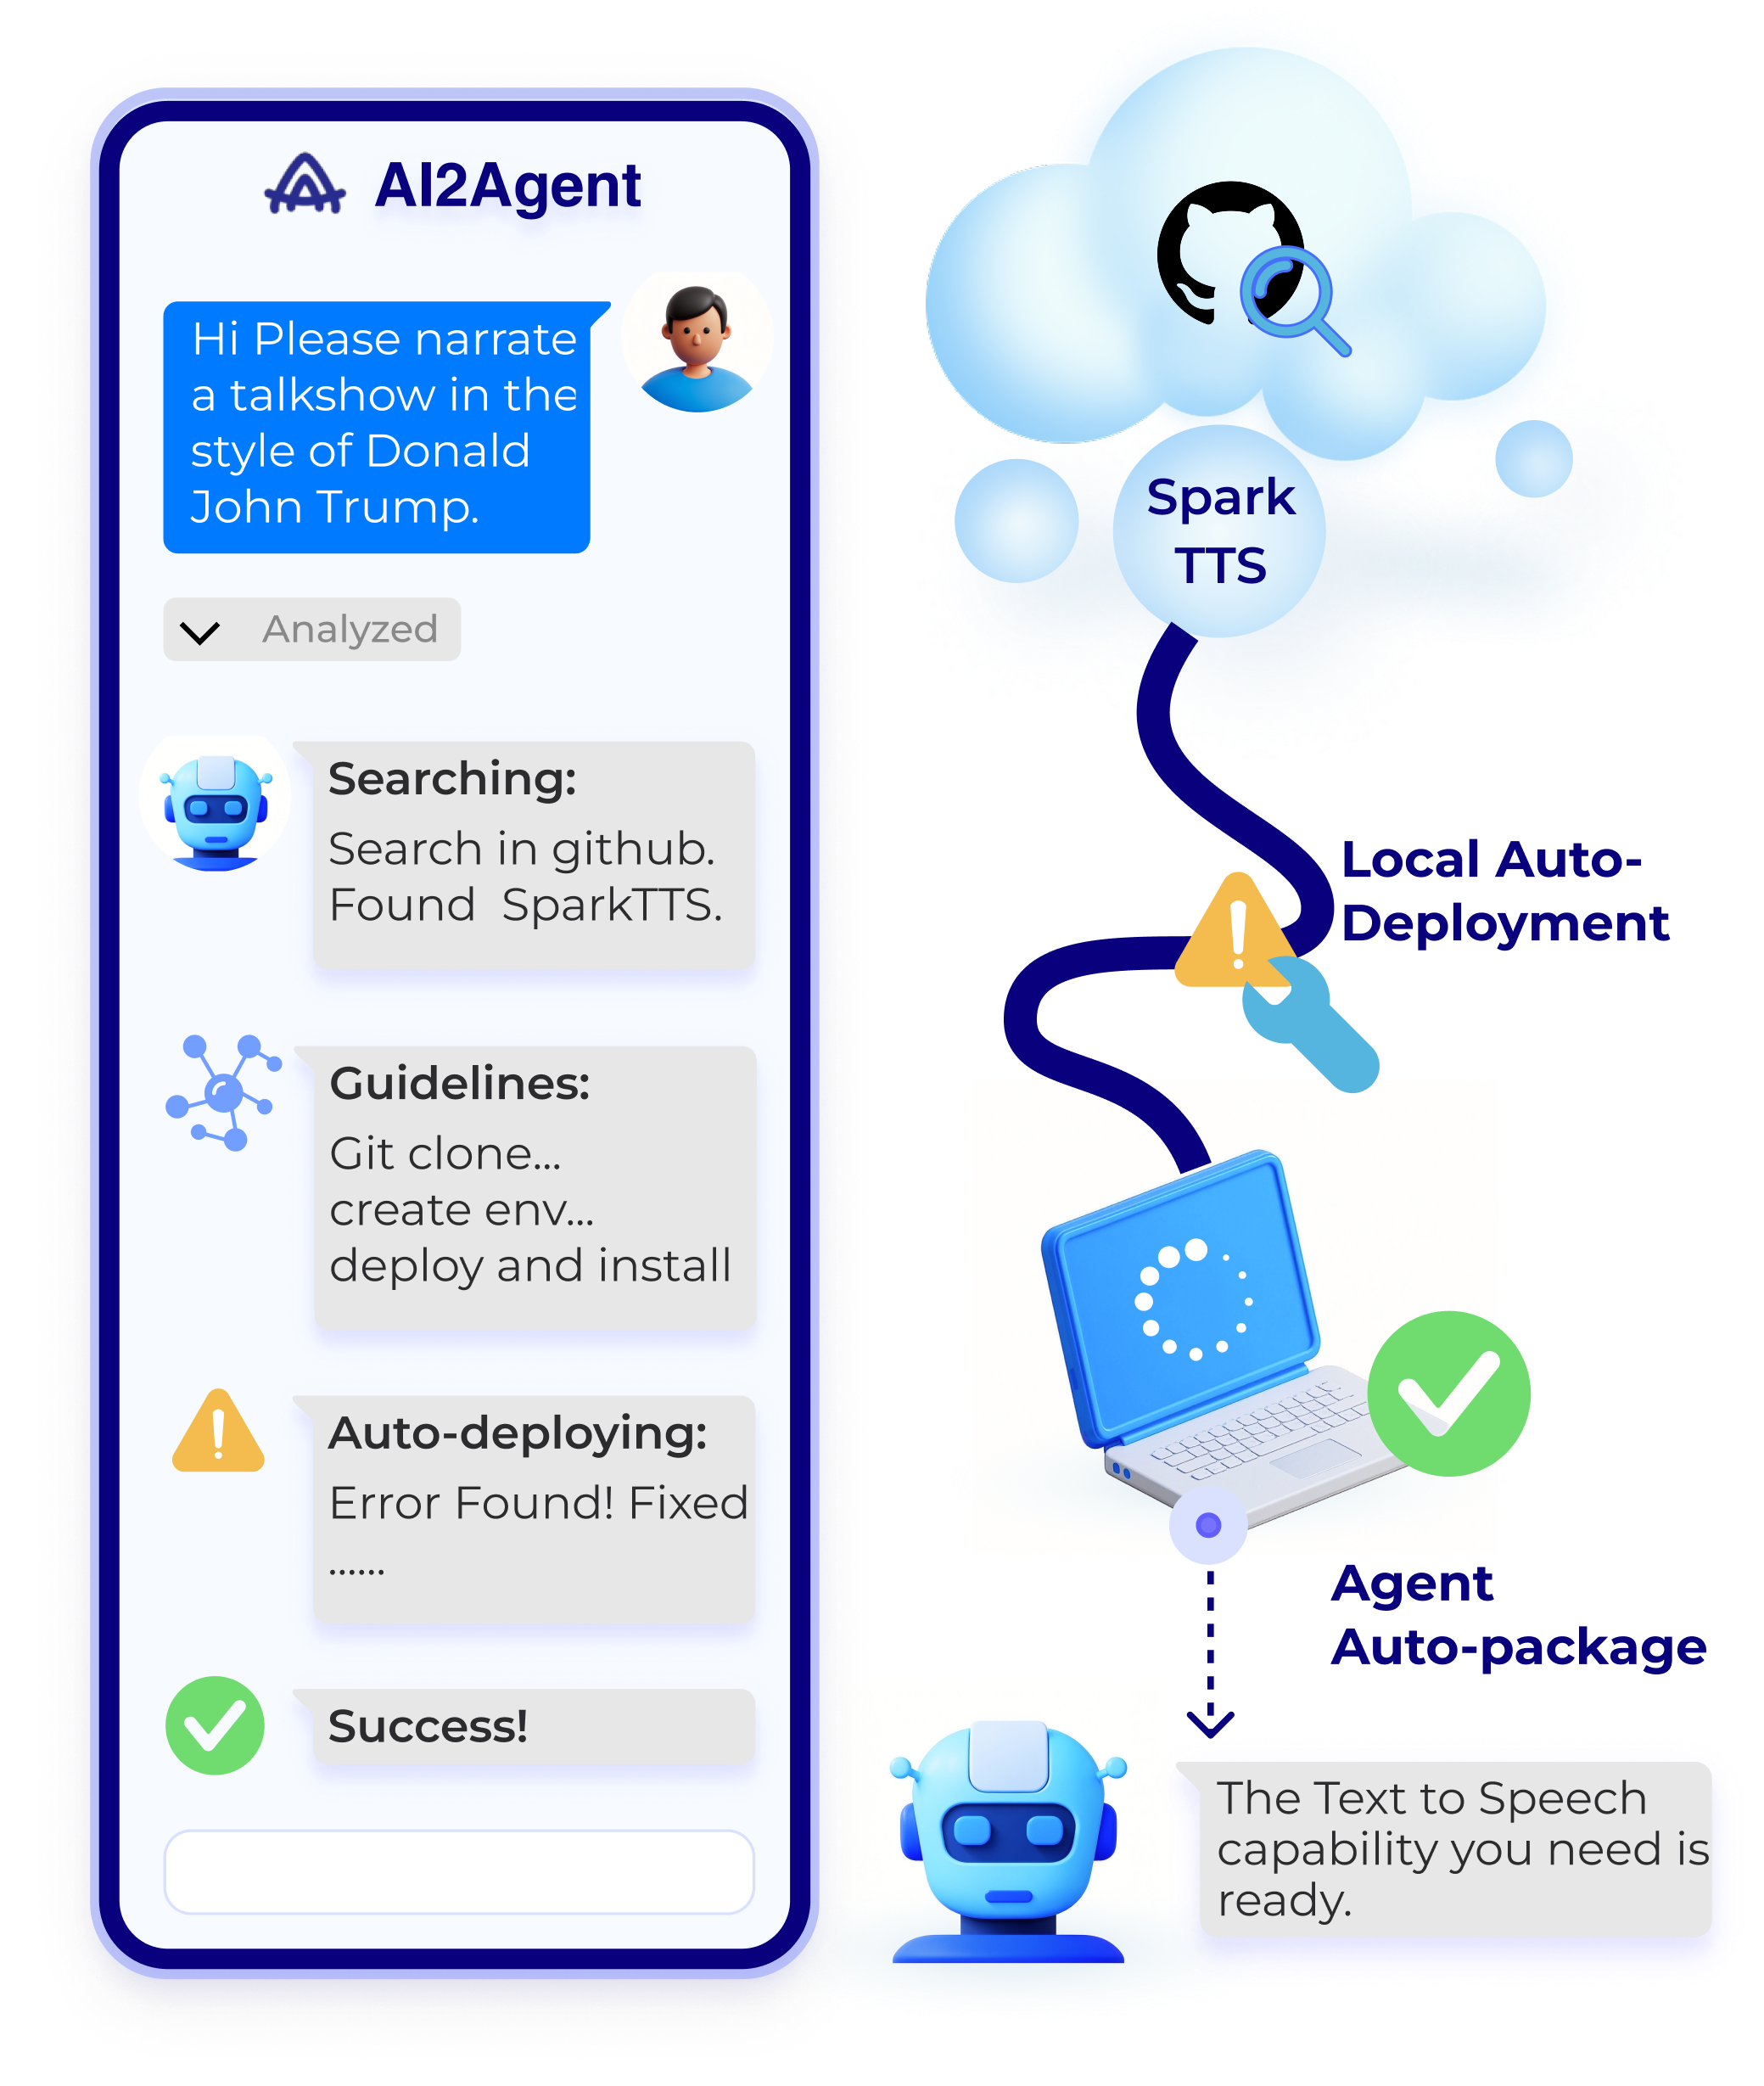
\includegraphics[scale=0.3]{imgs/value_proposal.png}
	\caption{
		\textbf{Left:} The AI2Agent user interface, illustrating the automated workflow where a user request (e.g., generating a talk show in a specific style) initiates a structured execution process. This includes searching for a suitable project, following the predefined guidelines for execution, auto-deployment and debug to ensure success.  
		\textbf{Right:} A conceptual visualization of local auto-deployment and Agent auto-package, demonstrating how AI2Agent transforms text-to-speech(TTS) functionality into a fully autonomous agent.
	}
	\label{fig:value}
\end{figure}

AI is revolutionizing industries, from autonomous driving to healthcare and finance. However, to fully realize its potential, AI must be effectively deployed into diverse environments. Deployment remains a major bottleneck due to complex environment configurations, dependency conflicts, and cross-platform adaptation issues, which hinder scalability and adoption.By automating deployment and debugging, AI can be more efficiently integrated across diverse domains, reducing engineering barriers and accelerating innovation at scale.

Automated deployments in industry predominantly follow DevOps paradigm~\cite{bass2015devops,ebert2016devops}, where execution environments, dependencies, and orchestration rules are defined using static configuration files (e.g., YAML). In this approach, developers manually configure environments, specifying software packages, version constraints, and computational resource allocations. CI/CD pipelines are then employed to automate building, testing, and deployment. To enhance automation, tools like AutoDevOps~\cite{AutoDevops} utilize predefined templates that streamline the configuration process. 

However, these methods have significant limitations. First, they lack flexibility, as they cannot adjust deployment strategies based on runtime conditions. This often leads to manual fixes for dependency conflicts, environment mismatches, and hardware compatibility issues. Second, they fail to retain and reuse past solutions, meaning each deployment starts from scratch. Developers must repeatedly troubleshoot the same problems, making the process inefficient and time-consuming. Third, they do not support scalable AI workflows, as they focus on deploying isolated models rather than integrating multiple AI components. Real-world AI applications often require chaining models or services together, but without standardized interfaces, these tools cannot effectively automate such tasks. As a result, deployment remains fragmented, difficult to scale, and heavily dependent on manual intervention.

To overcome these limitations, we introduce AI2Agent, an end-to-end framework that transforms AI projects into Autonomous Agents, enabling adaptive and reusable deployments. Unlike static DevOps paradigm, AI2Agent leverages autonomous execution, real-time debug, and experience accumulation to stabilize deployment processes.It consists of three components: Guideline-driven Execution, Self-adaptive Debug, and Case \& Solution Accumulation. Guideline-driven Execution ensures repeatable and structured deployments by following predefined guideline steps, such as searching for dependencies and executing system commands. Unlike static scripts, AI2Agent adapts dynamically to various environments. Self-adaptive Debug enhances deployment reliability by adjusting strategies based on real-time feedback, autonomously troubleshooting issues like search online or query the knowledge repository. Finally, Case \& Solution Accumulation utilizes a Knowledge Repository and RAG~\cite{graphrag,lightrag,ragflow}
to store past experiences, continuously refining deployment strategies and reducing errors, leading to more efficient deployments over time.

To validate the capabilities of AI2Agent, we conducted a case study on the automated deployment of multiple AI applications, including TTS~\cite{sparktts}, text-to-image generation~\cite{dall-e}, and image editing~\cite{instructpix2pix}. As shown in Figure~\ref{fig:value}, AI2Agent autonomously searches for and executes deployments, following predefined guidelines, and successfully packages them as Agents through self-adaptive debug. Test results show that AI2Agent significantly shortened deployment time, improved success rates, and reduced errors, leading to faster and more reliable deployments. This demonstrates its potential in enabling standardized, modular, and reusable AI deployments, paving the way for a more autonomous and interoperable AI ecosystem.

The key contributions of this paper are as follows:
\begin{itemize}
    \item We introduce \textbf{AI2Agent}, an end-to-end framework that automates AI project deployment by transforming them into autonomous Agents. It provides a standardized Agent interface, enabling modular management, seamless execution, and improved reusability, fostering a more interoperable AI ecosystem.
    \item Our approach comprises \textbf{Guideline-driven Execution, Self-adaptive Debug, and Case \& Solution Accumulation}, forming a structured yet flexible framework. It follows predefined guidelines while dynamically adapting to deployment environments and continuously improving through accumulated experience.
    \item We evaluate AI2Agent across \textbf{30 AI projects}, covering areas such as TTS, text-to-image generation, and image editing. Experimental results show \textbf{significant reductions in deployment time and error rates}, demonstrating the effectiveness and reliability of our approach in streamlining AI deployment.
\end{itemize}